\documentclass[border=3pt]{standalone}
% Preâmbulo compartilhado pelos diagramas TikZ da aula 6 de IHC (Necessidades e Requisitos)
\usepackage[T1]{fontenc}
\usepackage[utf8]{inputenc}
\usepackage{lmodern}
\usepackage{amsmath}
\usepackage{xcolor}
\usepackage{tikz}
\usetikzlibrary{arrows.meta,angles,quotes,decorations.pathmorphing,calc,
                positioning,shapes.geometric,shapes.misc,backgrounds,fit,
                math}

% Paleta (mesma dos SVGs originais)
% Paleta da disciplina de IHC: acento roxo (#755099), da capa do livro.
% (o nome "dblue" é mantido para não alterar todos os diagramas)
\definecolor{dblue}{HTML}{755099}
\definecolor{dorange}{HTML}{B3541E}
\definecolor{dgreen}{HTML}{4A7C59}
\definecolor{dred}{HTML}{9C4B4B}
\definecolor{dcream}{HTML}{F4F1EA}
\definecolor{dshade}{HTML}{DDD7C9}

% Função gaussiana (não normalizada por padrão de escala visual)
\pgfmathdeclarefunction{gauss}{3}{%
  \pgfmathparse{1/(#3*sqrt(2*pi))*exp(-((#1-#2)^2)/(2*#3^2))}%
}

% Estilos comuns (prefixo d... para não colidir com chaves internas do pgf)
\tikzset{
  >={Stealth[length=2mm]},
  dguide/.style={gray!55, dashed, line width=0.4pt},
  daxis/.style={gray!60, line width=0.7pt, ->},
  dbody/.style={fill=black!3, draw=black!80, line width=1pt},
  dacc/.style={draw=dblue, line width=1pt},
  dlbl/.style={black!55, font=\small},
  dsub/.style={black!45, font=\footnotesize},
  dstate/.style={circle, draw=black!80, fill=dcream, line width=1pt,
                 minimum size=17mm, font=\large, inner sep=1pt},
  dobs/.style={circle, draw=black!80, fill=dshade, line width=1pt,
               minimum size=14mm, font=\large, inner sep=1pt},
  dbox/.style={rounded corners=2pt, draw=black!80, fill=dcream, line width=1pt,
               align=center, inner sep=6pt},
  dop/.style={circle, draw=black!80, fill=white, line width=1pt,
              minimum size=6mm, inner sep=0pt, font=\small},
  dtrans/.style={->, dblue, line width=1pt},
  dmeas/.style={->, dorange, line width=1pt},
  dcurve/.style={line width=1pt, dblue},
  dcurveb/.style={line width=1.4pt, dorange},
}

\begin{document}
\hyphenpenalty=10000 \exhyphenpenalty=10000 \tolerance=9999 \emergencystretch=3em
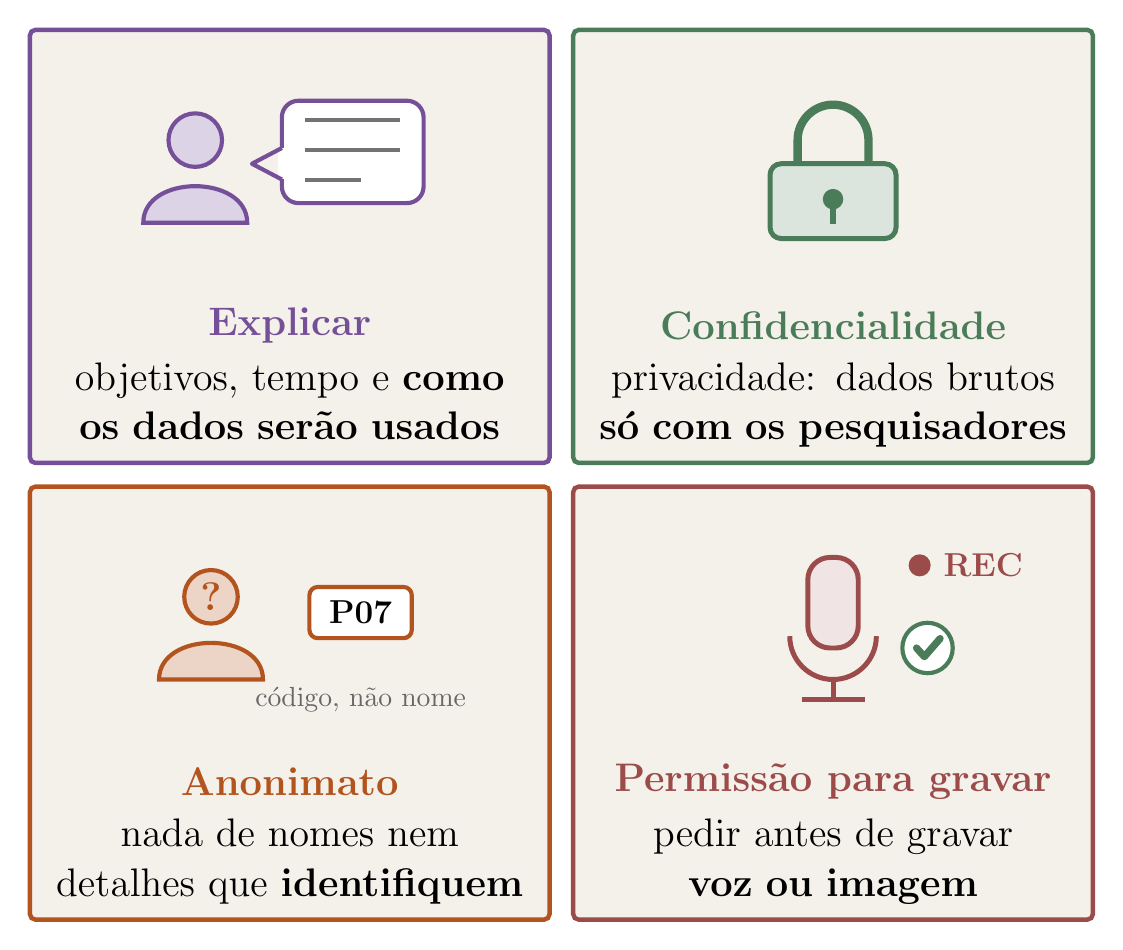
\begin{tikzpicture}[x=1cm,y=1cm]
\node[dbox, draw=dblue, line width=1.6pt, minimum width=6.6cm, minimum height=5.5cm] at (3.30,8.55) {};
\node[font=\Large\bfseries, dblue] at (3.30,7.55) {Explicar};
\node[font=\Large, text width=6.0cm, align=center, anchor=north] at (3.30,7.20) {objetivos, tempo e \textbf{como os dados serão usados}};
\fill[dblue!25!white, draw=dblue, line width=1.5pt] (2.10,9.90) circle (0.34);
\fill[dblue!25!white, draw=dblue, line width=1.5pt] (1.44,8.85) .. controls (1.44,9.47) and (2.76,9.47) .. (2.76,8.85) -- cycle;
\draw[dblue, fill=white, line width=1.5pt, rounded corners=6pt] (3.20,9.10) rectangle (5.00,10.40);
\draw[white, line width=2.6pt] (3.20,9.40) -- (3.20,9.80);
\draw[dblue, line width=1.5pt, line join=round] (3.20,9.40) -- (2.82,9.60) -- (3.20,9.80);
\draw[black!55, line width=1.4pt] (3.50,10.15) -- ++(1.20,0);
\draw[black!55, line width=1.4pt] (3.50,9.77) -- ++(1.20,0);
\draw[black!55, line width=1.4pt] (3.50,9.39) -- ++(0.70,0);
\node[dbox, draw=dgreen, line width=1.6pt, minimum width=6.6cm, minimum height=5.5cm] at (10.20,8.55) {};
\node[font=\Large\bfseries, dgreen] at (10.20,7.55) {Confidencialidade};
\node[font=\Large, text width=6.0cm, align=center, anchor=north] at (10.20,7.20) {privacidade: dados brutos \textbf{só com os pesquisadores}};
\draw[dgreen, line width=3pt] (9.75,9.55) -- (9.75,9.90) arc (180:0:0.45) -- (10.65,9.55);
\draw[dgreen, fill=dgreen!20!white, line width=1.8pt, rounded corners=4pt] (9.40,8.65) rectangle (11.00,9.60);
\fill[dgreen] (10.20,9.15) circle (0.13);
\draw[dgreen, line width=2pt] (10.20,9.10) -- (10.20,8.83);
\node[dbox, draw=dorange, line width=1.6pt, minimum width=6.6cm, minimum height=5.5cm] at (3.30,2.75) {};
\node[font=\Large\bfseries, dorange] at (3.30,1.75) {Anonimato};
\node[font=\Large, text width=6.0cm, align=center, anchor=north] at (3.30,1.40) {nada de nomes nem detalhes que \textbf{identifiquem}};
\fill[dorange!25!white, draw=dorange, line width=1.5pt] (2.30,4.10) circle (0.34);
\fill[dorange!25!white, draw=dorange, line width=1.5pt] (1.64,3.05) .. controls (1.64,3.67) and (2.96,3.67) .. (2.96,3.05) -- cycle;
\node[font=\Large\bfseries, dorange] at (2.30,4.10) {?};
\node[draw=dorange, fill=white, line width=1.5pt, rounded corners=3pt, font=\large\bfseries, minimum width=1.3cm, minimum height=0.65cm] at (4.20,3.90) {P07};
\node[font=\normalsize, black!60] at (4.20,2.80) {código, não nome};
\node[dbox, draw=dred, line width=1.6pt, minimum width=6.6cm, minimum height=5.5cm] at (10.20,2.75) {};
\node[font=\Large\bfseries, dred] at (10.20,1.75) {Permissão para gravar};
\node[font=\Large, text width=6.0cm, align=center, anchor=north] at (10.20,1.40) {pedir antes de gravar \textbf{voz ou imagem}};
\draw[dred, fill=dred!15!white, line width=1.8pt, rounded corners=8pt] (9.88,3.45) rectangle (10.52,4.60);
\draw[dred, line width=1.8pt] (9.65,3.60) arc (180:360:0.55);
\draw[dred, line width=1.8pt] (10.20,3.05) -- (10.20,2.80) (9.80,2.80) -- (10.60,2.80);
\fill[dred] (11.30,4.50) circle (0.14);
\node[font=\large\bfseries, dred, anchor=west] at (11.48,4.50) {REC};
\draw[dgreen, fill=white, line width=1.5pt] (11.40,3.45) circle (0.32);
\draw[dgreen, line width=2.6pt, line cap=round, line join=round] (11.26,3.45) -- (11.36,3.34) -- (11.56,3.57);
\end{tikzpicture}
\end{document}
